% !TEX root = ../thesis.tex
\chapter{Lit Review}
	\label{chap:lit_review}
	Education and the sharing of knowledge is a powerful tool. In fact, in our opinion the most important skill anyone can have. As a famous quote said, "give a man a fish, and he will starve, but teach him to fish, and he won't be hungry anymore". However, it wasn't until 1918 that education, as most people in England and Wales have experienced, started to come into effect \cite{education1918}.
	
	Education over the years was very much about just giving the knowledge to the students from the teacher. It wasn't until 1988, under the Education Reforms Act 1988, that assessments got introduced. The introduction was through the introduction of the national curriculum in England and Wales \cite{education1988}.
	
	As the curriculum got rolled out, statutory assessments got introduced to education between 1991 and 1995. Key Stage 1 first, followed by Key Stages 2 and 3, respectively \cite{hutchison1994reliable, dillon2011becoming}. Only for the core subjects of English, Mathematics and Science had the assessments first introduced. The first assessments in Key Stage 1 were a range of cross-curricular tasks to be delivered in the classroom, known as standardised assessment tasks - hence the common acronym 'SATs'. However, the complexity of the use of these meant more formal assessments quickly replaced them \cite{hutchison1994reliable, dillon2011becoming}. The assessments in Key Stages 2 and 3 got developed using more traditional tests.
	
	To allow teachers to judge students' attainment, taking tests became the main assessment form in key stage 3. While assessments were the main form, educators were also able to assess their students with other means against the targets set for attainment within the national curriculum \cite{dillon2011becoming}. The teacher and assessment outcomes got used on a scale with key learning milestones expected at different ages. A key stage level indicated the result for the students progress. The model was used throughout the next few years until 2005 when the role of tests in KS1 got downgraded to just being an internal support tool to teachers, and in then 2008, the government decided to remove tests in KS3 \cite{dillon2011becoming}.
	
	This model continued, with minor adjustments to reflect the changing content of the National Curriculum, up to 2004. From 2005, the role of the tests got downplayed at Key Stage 1, with tests being used only internally to support teacher assessment judgements \cite{bbc_no_tests}. Further changes came in 2008 when the government announced that testing in Key Stage 3 was to get scrapped altogether \cite{bbc_tests_scrapped}.
	
	However, with a change of government party, the Conservative party taking power from the Labour party brought about new changes to how education's focuses and pedagogy methods would get conducted. In 2014 the system of attainment levels was removed, creating the educational shift of "Assessing without level" \cite{ass_without_lvls}. However, within schools, it was being referred to as 'life after levels'. Especially by our educational colleges and us at the time. Which was the follow up to the changes in the national curriculum in 2013 \cite{ass_without_lvls}. The changes within the national curriculum brought a greater focus on more traditional style GCSE academic subjects while reducing the focus on perceived technical labour style jobs. The new curriculum direction created more emphasis on the final exam outcomes at the stages of GCSE and A-Level.
	
	\section{The Purpose of Assessment, Marking and Feedback in Education}
	As we have established, assessments became a staple of the UK educational system in 1988. While the term assessments are not usually defined, the word 'assess' is typically associated with measuring, determining, evaluating, and judging \cite{wellington2007secondary}.
	
	While there can be multiple reasons why educators assess students, assessments aim to serve a purpose to both the teacher and the student in the process. These include: giving feedback to teachers and learners; providing motivation and encouragement; to boost the self-esteem of the pupils; a basis for communication; a method to evaluate a lesson/training method/scheme of work/ curriculum; to entertain \cite{wellington2007secondary}. Additionally, the assessment also creates other opportunities to rank students; a method to select and filter students, allocate students a particular pathway or educational direction, or as a way to discriminate or choose between students for a given set reason \cite{wellington2007secondary}.
	
	\subsection{Traditional Methods of Assessment and Feedback} % Should these be subsections?
	There are four main categories of assessment. These are diagnostic, formative, summative, and national assessments \cite{wellington2007secondary, dillon2011becoming}. However, it is essential to note that national assessments do not get used within everyday aspects of teaching and learning. This term is the name given to the critical exams like SATS, GCSE and ALevel exams taken nationally. Therefore we will focus on the other three main ones.
	
	Diagnostic assessment is what gets referred to as pre-testing \cite{wellington2007secondary}. Educators use this technique to get a base level of knowledge of the students they have inherited. This method is good for showing the progress of attainment over time by having an initial base test. Teachers can then show how well the students have progressed over time with their improvements over the term. This base assessment also provides the teacher with crucial information - the current ability of every student's knowledge. Through knowing this current level of knowledge, teachers can adapt the coming lessons and provide suitable differentiation and scaffolding within the lessons to allow each student to succeed as much as possible. However, we also experienced, within our time as an educator, the technique getting used to create baseline narratives. Teachers were using them to show that the student's knowledge wasn't at the expected level when inherited by the teacher at meetings or performance management reviews. Therefore, being used as a counter-act measure tool by the teacher, if they find themselves being accused of letting the students' performance slip, by trying to counter-act by implying the students were not at the required level in the first place.
	
	The second method, formative assessment, is also known as 'assessment for learning (AFL)' \cite{wellington2007secondary, dillon2011becoming}. This method has become one of the main tools for a teacher in terms of assessment and feedback. AFL allows the educator to assess the students' understanding of a topic on the fly during a lesson without a summative assessment. As a result, allowing the teacher to spend more or less time if the students do or don't get the topic, even if they planned more or less time for that topic. Therefore, ensuring that the teaching is not getting carried out for teaching sake. Thus, the emphasis is less on measurements and more on actual learning. AFL can involve using several techniques: teacher assessment - through in-class questions, marking books; to the students assessing their work called self-assessment, or peer assessment - where the students evaluate each other's work \cite{wellington2007secondary}.
	
	AFL has many values for teachers and students. Within Black and William's paper. 'Inside the black box \cite{black1998inside}' discovered that AFL provides massive learning gains, especially with the low attainer groups. Black and William found that AFL and the use of peer assessment raised motivation and self-esteem across the board, but even more so in the low attainers. With the addition of peer assessment being extra valuable to the students. This form of feedback is effective as the feedback will most likely be given back to the students in a manner that they are more familiar with, informs of language and wording. Therefore in a way that makes more sense to them and having the most impact on their learning \cite{torrance1998investigating, black1998inside}.
	
	The two key ways that teachers can gain insights from AFL is in questioning and marking. Questioning, also referred to as formative questioning, aims to assess what the students in the classroom know about the current topic being discussed or taught to improve learning \cite{wellington2007secondary}. However, for this to be effective, students will need an appropriate 'wait time' \cite{black2001feedback}. A 'wait time' is the term used to ensure that the student, when asked a question, has to be able to formulate their thoughts and answer as the aim is not to catch them out but to gather what they currently understand. Formative questioning is also good when allowing the students to discuss amongst themselves, then answer the teacher. Therefore, allowing them to consolidate with peers to check if they understand the topic before delivering it to the teacher. A student is more likely to say they do not know than give a wrong answer and look silly in front of their peers, known as the technique 'think-pair-share'. Other effective techniques, which do not require students to discuss between themselves, are 'no-hands up', 'show-me board', 'traffic light' systems \cite{oecd}. 
	
	Formative marking is the term used when teachers mark students' work and provide some form of feedback, whether it be two starts and a wish or more standard approaches of providing straight-up feedback. The overall aim is to allow the teacher to see where the student is within their knowledge, gain a level of where they are at and then provide feedback of what they have done well but ultimately what they need to improve on. The proving feedback on areas to improve on are essential whether the student is at a C/4 or an A*/9. The constant feedback, no matter the students level, is as an educator always aims to ensure their students can do better. However, it is crucial that the feedback is taken on board and actioned for formative marking to be effective. Otherwise, it is more of a summative action \cite{black1998inside, william1990national}. To combat this, educators would usually allow students times within a lesson, after the feedback gets given, to go back over their work and make changes to their work in a different colour.
	
	The third method is a summative assessment, also known as 'assessment of learning (AOL) \cite{wellington2007secondary}. This type of assessment happens at the end of a teaching unit or topic. It gets used to gain insights into what the students have learnt within the subject covered or the course. Its purpose is to give a student a mark, grade or ranking. Usually, this is the grade that is mainly focused on, as it is the metric that will impact the school the most in terms of league performance tables regarding GCSE and A-level results. From our experience, summative assessments are carried out regularly within schools. This assessment method tends to get used to getting a snapshot of the students of whit if a moment like, if they were to take the test now, what would they get? By seeing the results, educators can see if students need to attend intervention or if they are performing as expected or even better. With so much riding on these results, for schools and teachers performance management reviews, a lot of emphasis on put into trying to predict the final results for students. We have seen it put a lot of pressure on the teachers and the students and ultimately creates a very stressful environment, which is not the best environment for learning.
	
	
	
	
	\subsection{Why Traditional Traditional Marking and Feedback Methods are Effective}
	
	
	\subsection{The Negative Aspects of Traditional Marking and Feedback Methods}
		
		While marking and feedback are essential in a classroom, they also bring about some negative aspects. As debates are happening about who formative assessment is really for \cite{wellington2007secondary}, are these assessments for the students done to allow the students to be able to improve on their work and knowledge. Or are they more for the schools to predict actually where the students will be, come exam time. Or are they there to show external bodies, like Ofsted, that the school is being rigorous. Or are they for teachers to justify possible results based on results for their performance management reviews?
		
		Additionally, as teachers might have had a KS4 (GCSE) class for two to three years when assessing and doing the summative assessment, the teacher might not see that student's work entirely at face value. The teacher's personal bias might jump in based on how the student has been over the year or even years. For example, if one student has been nice, well behaved and just done the required work, the teacher might provide a higher grade for that student. However, they might give a lower grade score for someone who has been a pain and misbehaved through the year. However, the second student's work might be of better quality, but it is not seen at face value and therefore not accurately marked because of the other factors.
		
		As schools might have multiple teachers teaching a particular subject simultaneously, a process called moderation is required. Moderation aims to make sure that all work being marked and graded is all at the same level. For example, teachers A, B and C's student's work, awarded a Distinction *, are all at the exact agreed and expected quality. However, this can bring about multiple issues. One is that not all teachers might interpret the mark scheme the same as the others and therefore look for different attributes within the students' work. While moderation and standardisation aim is to find out these inconsistencies and get all the teachers on the same page regarding expectations, office politics can also hugely impact it. Imagine the scenario. Five teachers are teaching the same year group and qualification. One teacher is the lead to that subject, so, therefore, would have had all the required training from the exam boards regarding the course, another one is a regular teacher. At the same time, one is an assistant principal, another is a vice principal, and the final one is the head of the faculty. So in the whole school context, the subject lead teacher is higher in the hierarchy than the regular teacher but lower than the other three. However, in the scope of the qualification getting delivered, the lead teacher is at the top. But this can bring about the office politics we were alluding to. Some teachers who are higher up in the school system but not in the qualification scope can throw their weight around say things need to be how they have interpreted the mark scheme. Their interpretation is not always correct, but they push their view for whatever reason, bringing about a few situations. Resulting in, will the lead teacher challenge the more senior figure to say that they are wrong and the exam board expects this, or will they agree not to upset the more senior member of staff? Either way might not end well, and with the tricky world of education, the second option is the more likely choice. However, this brings about issues in regards to inconsistency with work and the awarded mark.
		
		Another drawback to traditional marking is that the requirement of personalised feedback for students. To allow them to develop, students must have personalised areas of where they need to improve. However, in controlled assessments, teachers can give feedback, but it can not be personalised. It has to be generic, but most schools' policies require the feedback to be personalised, creating a conflict between the exam board's requirements and the school's requirements based on Ofsted's expectations. The situation makes a moral and ethical decision. They are likely to be reprimanded by the school if they do not provide the feedback but can be done for malpractice if the exam board catches them for giving the feedback.
		
		When a summative assessment has occurred within a learning sequence, students get usually presented with a grade and feedback. This feedback and mark could be for the end of unit exams or homework, for example. While the teachers want students to focus on the feedback given to help them improve, students focus on the results and will naturally rank order themselves. The UK government has attempted to try and resolve this by removing levels in KS3. However, when KS4 focuses on the final summative assessment, their actual GCSE exams, a provided grade is hard not to offer. Therefore, it is vital to make sure that feedback is acted upon once given.
		
		Finally, a big issue in regards to marking and providing feedback is time. It takes a long time to score a students' work and then give feedback to the students. It is also a very tedious task that a teacher might not do in one sitting. Therefore, with many potential variables in play, the marking of the points award per each exam question, for example, might not be the same. There is also a massive cognitive load that is placed upon the teacher while trying to mark.
		
		Consequently, it is challenging to ensure that consistency and fairness are not playing a part in the marking. However, the enormous cognitive load placed upon the teacher can be very draining. It can then affect the quality of the teachers delivery within the lesson, especially with the stress aspects that get placed upon them regarding how quick the feedback needs to get returned to the students.
	
	\section{Comparative Judgement}
	
	
	\subsection{What is Comparative Judgement} 
		Comparative judgement is a mathematical way to determine which observation item is better than the other item also being observed compared to each other. This method was first proposed in 1927 by Louis Leon Thurstone, a psychologist, under the term "the law of comparative judgement" \cite{thurstone1927psychophysical, thurstone1927law}. In modern-day terminology, it gets more aptly described as a model used to obtain measurements from any pairwise comparison process. Examples of such methods are comparing the perceived intensity of physical stimuli, such as the weights of objects, and comparing the extremity of an attitude expressed within statements, such as statements about capital punishment. The measurements represent how we perceive things rather than being measurements of actual physical properties. This kind of measurement is the focus of psychometrics and psychophysics. <wikipedia>
		
		In more technical terms, the law of comparative judgment is a mathematical representation of a discriminal process. This process involves a comparison between pairs of a collection of entities concerning multiple magnitudes of attributes. The model's theoretical basis is closely related to item response theory and the theory underlying the Rasch model. These methods are used in psychology and education to analyse data from questionnaires and tests.
		<wikipedia>
		
		While comparative judgement is a technique that has been around for almost 100 years, it wasn't until the early nineties that this technique got proposed for use within an educational setting. This first proposal was by Politt and Murry \cite{pollitt1996raters}, who conducted a study where they tested candidates on their English proficiency within Cambridge's CPE speaking exam. The judges watched 2-minute videos and judged which one out of a pair of videos they deemed better at the requested task in the exam. However, before this, in the ninety seventies and eighties, comparative judgement was presented as a more theoretical basis for educational assessments \cite{andrich1978rating}. 
		
		With the momentum of his findings, Politt then presented comparative judgement as a tool for exam boards to use to be able to compare the standards of A-Levels from the different exam boards, replacing the direct judgement of a script that was at the time currently being used \cite{newton2007paired}. In his papers titled, "Let's Stop Marking Exams" \cite{stop_marking_pollitt}, he presents a valid argument for using comparative judgement, with the advantages it brings over some traditional types of marking.
		
		Politt, in 2010, also presented a paper at the Association for Educational Assessment – Europe. It was about How to Assess Writing Reliably and Validly. Politt presented evidence of the extraordinarily high reliability achieved with Comparative Judgement in assessing primary school pupils' skill in first-language English writing \cite{pollitt2009abolishing}.
		
	\subsection{The Logic Behind Comparative Judgement and What it Aims to Do} % Should these be subsections?
		How comparative judgement works is to present two options to a marker. The marker then gets asked to pick which one of the two options they think is the better one. The marker will get presented with all possible combinations available, each time picking which one they think is the better one out of the two. An outputted score is then presented based on the method used. The original method, the Law of Comparative Judgement (LCJ), follows the formula:
		
		\begin{figure}[h]
			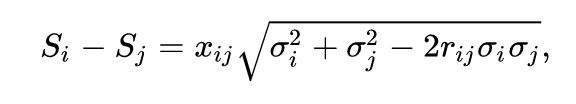
\includegraphics[width=8cm]{graphics/LCJ_formula.png}
			\caption{}
			\centering
		\end{figure}
	
		 $S_{i}$ is the psychological scale value of stimuli $i$
		%{\displaystyle x_{ij}} is the sigma corresponding with the proportion of occasions on which the magnitude of stimulus i is judged to exceed the magnitude of stimulus j
		%{\displaystyle \sigma _{i}} is the discriminal dispersion of a stimulus {\displaystyle R_{i}}
		%{\displaystyle r_{ij}} is the correlation between the discriminal deviations of stimuli i and j
		%The discriminal dispersion of a stimulus i is the dispersion of fluctuations of the discriminal process for a uniform repeated stimulus, denoted {\displaystyle R_{i}}, where {\displaystyle S_{i}} represents the mode of such values. Thurstone (1959, p. 20) used the term discriminal process to refer to the "psychological values of psychophysics"; that is, the values on a psychological continuum associated with a given stimulus.
		
		However, an alternative version derived from Louis Leon Thurstone, referred to as the "Pairwise Comparison" \cite{thurstone1927law}, will provide an output based on the difference between the quality values is equal to the log of the odds in respect to object-A will be object-B. This formula gets represented as: 
		$\displaystyle \mathrm {log\;odds} (A\ {\text{beats}}\ B\mid v_{a},v_{b})=v_{a}-v_{b} $.
		
		$\Pr\{X_{ji}=1\}={\frac {e^{{\delta _{j}}-{\delta _{i}}}}{1+e^{{\delta _{j}}-{\delta _{i}}}}}=\sigma (\delta _{j}-\delta _{i})$
		
		 .
		%\displaystyle \mathrm {log\;odds} (A\ {\text{beats}}\ B\mid v_{a},v_{b})=v_{a}-v_{b}}		


	\subsection{How effective is Comparative Judgement at Providing Feedback?} % Should these be subsections?
		
	
	\section{Other Rating Systems}
	While comparative judgment has proven to be a suitable method of ranking pairwise matches of students work over the years, it has its limitations. For example, comparative judgment requires every combination to be compared against, which means for a class of thirty students, accounting for four hundred and thirty-five different combinations. Take into account a subject like English, which every student will have to take. A typical school year could have one hundred and twenty students, which would mean seven thousand one hundred and forty different combinations. That is a lot of time and comparisons that would be required. Therefore, to truly take the cognitive load off a marker or teacher, it would be better to try and have different people sub-sample the work. Then, from the scoring of the sub-samples, use this to generate an overall ranking. In essence, it is creating a competitive scoring system against each other. Two suitable systems to achieve this would be an Elo or Glicko rating system.
	
	\subsection{Elo Ranking System}
	The Elo ranking got first introduced into competitive chess in the 1980s \cite{weng2011bayesian}. However, it got created in the 1960s by Arpad Elo as a replacement for the Harkness System. The Harkness System got used by the United States Chess Federation (USCF) at that time \cite{elo1978rating}. Additionally, the Elo system has gets used as a ranking system for football, American football, basketball as well as eSports like Counter-Strike: Global Offensive and League of Legends \cite{silver2015we, pradhan2020power}.
	
	The Elo system looks at the difference in two players ratings, then serves as a predictor for the match's outcome. The players Elo rating is depicted as a number and will change over time depending on the games' outcomes, with the winners taking points from the losers. However, how many points get awarded is decided upon the difference in ranking between the players. If the higher ranked player wins, only a few rating points get taken from the lower rank player. However, if an 'upset win' occurs, when the considerably lower rank player beats the higher rank player, then a much greater number of points will be gained to the winner and deducted from the loser. Ultimately, even when 'upset wins' happen, the ranking of the players will reflect the valid scores over time. [find reference]
	
	However, there are ways that players who know how the system works can cheat it. These methods include protecting one's rating, selective pairing and ratings inflation and deflation.
	
	Players protecting one's rating discourages game activity for players wanting to preserve their score. In essence, this situation gets created when players are not playing any more games once they are at a high score \textbf{[23]}.  A method against this behaviour is to award an activity bonus that gets combined with the ranking score \textbf{[24]}.
	
	Selective pairing is when players choose their opponents, which results in players choosing opponents that the player has the minimal risk of losing. Additions like a k-factor got added, but these do not solve the problem completely. \textbf{[find reference]}. Additional implementations have been added, like auto-pairing, which are based on random pairings but have a winner stays on context.\textbf{ [find reference]}.
	
	Inflation is when a score means less over time. For example, a player has a score of 2500 and gets ranked 5, but later, another is ranked 15. It is showing that the player's ability is decreasing over time. When deflation happens, this indicates that advancement is happening. Deflation is when a score of 2500, got a player ranking of 7, but at a later date, the score is then put ranked the player 2. Therefore, we must consider when using ratings to compare players between different eras. The ranking gets made more difficult when inflation or deflation are present. %(See also Comparison of top chess players throughout history.)

	The Elo system has a flaw in that it is almost certainly not distributed as a normal distribution. As a result, weaker players have greater winning chances than Elo's model predicts.\textbf{[citation needed]} However, the Elo ratings still provides a valuable mechanism for giving a rating based on the opponent's rating.
	
	\subsection{Glicko Ranking System}
	\textbf{The Glicko rating system and Glicko-2 rating system are methods for assessing a player's strength in games of skill, such as chess and Go. It was invented by Mark Glickman as an improvement on the Elo rating system, and initially intended for the primary use as a chess rating system. Glickman's principal contribution to measurement is "ratings reliability", called RD, for ratings deviation.}
	
	\textbf{Both Glicko and Glicko-2 rating systems are under public domain and found implemented on game servers online (like Pokémon Showdown, Lichess, Free Internet Chess Server, Chess.com, Online Go Server (OGS),[1] Counter Strike: Global Offensive, Team Fortress 2,[2] Dota Underlords, Guild Wars 2,[3] Splatoon 2,[4] Dominion Online and Gods Unchained,[5]), and competitive programming competitions. The formulas used for the systems can be found on the Glicko website.
	}
	\textbf{The RD measures the accuracy of a player's rating, with one RD being equal to one standard deviation. For example, a player with a rating of 1500 and an RD of 50 has a real strength between 1400 and 1600 (two standard deviations from 1500) with 95\% confidence. Twice (exact: 1.96) the RD is added and subtracted from their rating to calculate this range. After a game, the amount the rating changes depends on the RD: the change is smaller when the player's RD is low (since their rating is already considered accurate), and also when their opponent's RD is high (since the opponent's true rating is not well known, so little information is being gained). The RD itself decreases after playing a game, but it will increase slowly over time of inactivity.}
	
	
	\section{Natural Language Processing (NLP)}
	Natural Language Processing (NLP) is a subfield of AI that aims to understand natural language through trying to process and analyse it \cite{vasiliev2020natural, vajjala2020practical}. Ultimately NLP is teaching computers how to understand humans in natural language. However, this is not straightforward, as language is a complex, ever-changing form even for humans. There are three main categories that NLP problems fall into, heuristics, machine learning, and deep learning \cite{vajjala2020practical}. The nature of ML algorithms gets designed to work with unknown datasets, allowing data scientists to learn how to use language \cite{vasiliev2020natural}. While this will bring us a vast amount of insights, as mentioned before, the ever caning landscape of language does not mean that it is perfect and, once made, doesn't need revision. Therefore generating and understanding natural language are the most promising but most challenging tasks in NLP \cite{vasiliev2020natural, vajjala2020practical}.
	
	To understand the complexities of machines attempting to understand language, we must first know what we mean when we state 'what is language'. Language is a structured communication system, which involves many combinations of its fundamental components of varying complexities. For example, some of these components are characters, words and sentences to name a few \cite{vajjala2020practical}.
	
	Human language gets constructed of four major building blocks, and are phonemes, morphemes, lexemes and syntax, and context \cite{vajjala2020practical}. To make an effective NLP app, we need to ensure our application has these different building blocks used within its foundations (see fig: \ref{fig:practical_building_block}). However, knowing these building blocks does not entail we can do what we like within NLP. NLP has a lot of challenges that involve ambiguity, common knowledge, creativity and diversity across languages \cite{vajjala2020practical}. 
	
	\begin{figure}[t]
		\centering
		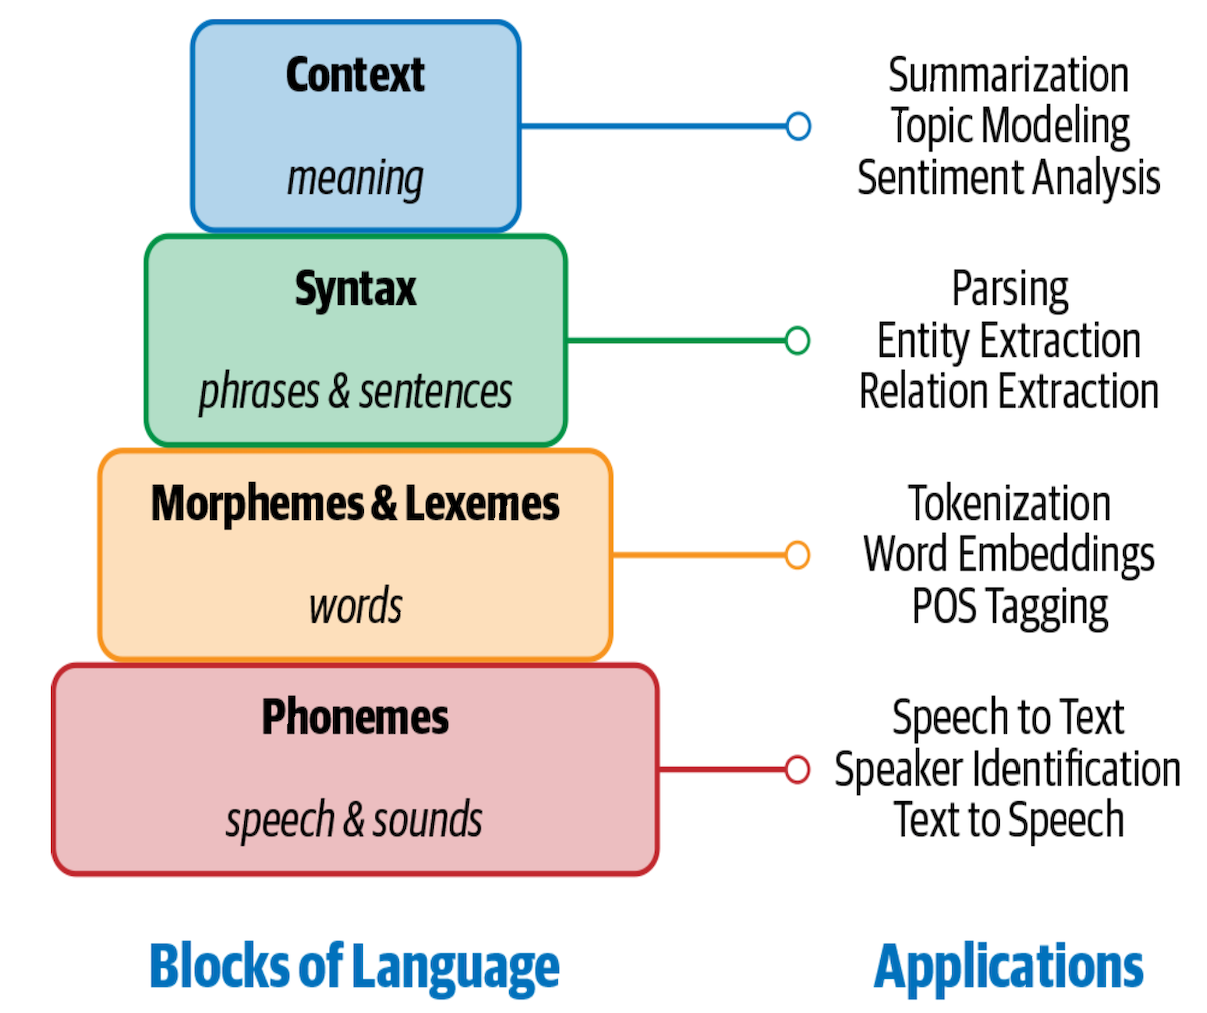
\includegraphics[width=8cm]{practical_building_block.png}
		\caption{The building blocks and their tools for understanding language \cite{vajjala2020practical}.}
		\label{fig:practical_building_block}
		
	\end{figure} 
	
	\section{Related Work}
		\label{sec:google_fu}
		
		While comparative judgment is not a new concept, only a few current systems implement a version of it as a tool for marking. These current CJ projects have a slightly different take on the CJ process but have very similar fundamentals. The current offerings are created or provided by RM Compare, a consortium of universities called D-PAC, No More Marking and e-scape.
		
		RM Compare is probably the version with the most prominent presence. 
		
		RM Compare uses Adaptive Comparative Judgement (ACJ), based on The Law of Comparative Judgement. The assessor (a teacher, lecturer, examiner or student) is presented with two anonymised pieces of work in a side-by-side pairwise comparison and asked to use their professional judgement to select which of the two is better at meeting the assessment criteria.
		
		RM Compare says that through repeated pairwise comparisons, optimised by an iterative, adaptive algorithm, a highly reliable scale or rank order is created through consensus over what 'good', 'better', and 'best' looks.
		
		%[Pros]
		RM Compare empowers users across educational organisations to collaborate on assessments and is proven to increase student attainment. It also reduces the cognitive load from teachers, which gets achieved through the very nature of the comparative judgment process. It also has a straightforward and effective UI for the user to interact with.
	
		%[cons]
		However, it still has an extensive workload as for it to be effective, the markers (known as judges) need to go through several rounds. Multiple examples online were stating 16 rounds. RM Compare states that these numerous rounds are required to reduce the error uncertainty rate.  The algorithm's adaptiveness will ensure that pairs closely matched to each other get checked more to confirm the order is correct, reducing the algorithm's error rate calculation. A high level of uncertainty will get compared more often to check the consensus between the judges. 
	
		An issue with the application is that it doesn't provide any real form of meaningful feedback. RM Compare suggests that the students gain feedback from the system is for the students to compare their peer's work through the system. Once this comparison by the students gets completed, the students' peered work ranking results will get compared against the teachers. Which then, in turn, gets used as a point of discussion. Therefore, in our opinion, not providing any meaningful form of feedback. While RM Compare that the process has a considerable impact on students attainment, this claim feels more like a marketing gimmick. While we agree that this process can generate insights into students' expectations, it does not provide meaningful, personalised feedback. Therefore, not allowing them to know what they need to do to improve.



	\subsection{Subsection all similar work}
		\label{sec:resources_bibtex}
	


	\subsection{Comparison of similar work}
	
	\section{Overall Aim}
	Comparative judgement is a power tool. It can remove a lot of cognitive load from the teacher. It also eliminates the teacher's bias in the marking process, especially when the teacher knows whose student they are marking. Teachers can consider how the student has performed over the year instead of how they did in that final piece of work.
	
	However, the current process of adaptive comparative judgment can reduce the cognitive load with the teacher marking and lessen the potential for bias from the teacher. Current implementations do have their limitations and still create a lengthy process. With some systems still having markers to mark student's work up to, some examples have 16 rounds of marking, which is still very time-consuming. Which, if you want to expand this to a national level, wouldn't be very effective.
	
	Therefore, we want to look into different methods of student work ranking orders that could get used to allowing a crowdsourced way of marking in a comparative judgement style, can be implemented. Suggested alternatives are an Elo system ranking. Additionally, we want to create NLP tools that will allow us to interrogate the data and see if there are any patterns within the data and the end rankings. Allowing us to suggest what aspects of the data makes the content get perceived as good.
